\documentclass[10pt,red]{beamer}

\usepackage[utf8x]{inputenc}
\usepackage{default}
\usepackage{presentation}
\usetheme{Warsaw}

\usepackage{presentation}
\usepackage{wrapfig}
\usepackage{fancyhdr}
\usepackage{mdwlist}
\usepackage{listings}
\usepackage{listing}

\usepackage{color}
\usepackage{textcomp}
\definecolor{listinggray}{gray}{0.9}
\definecolor{lbcolor}{rgb}{0.9,0.9,0.9}

\lfoot{Philips}
% =============================================================================
% All text contained in this cell can be put in another file say, titlepage.tex
% and can be included right here as % =============================================================================
% All text contained in this cell can be put in another file say, titlepage.tex
% and can be included right here as % =============================================================================
% All text contained in this cell can be put in another file say, titlepage.tex
% and can be included right here as \include{titlepage}
\title{Digital Logic Circuit Simulator}
%\subtitle{EES 401 Seminar}
\author[Group - 13]{%
Group Members:\\
Meghanad Shingate (09307608)\\
Nirbhay Rane (09307905)\\
Bharat Kumar (09307904)\\
% 09307608\\
% Guide : Prof.Abhay Karandikar
}

\institute[IIT Bombay]{%
% \vspace{-0.3in}
% % \begin{figure}
% % \begin{center}
% % \includegraphics[width=1.5cm]{iitblogo.png}
% % \end{center}
% % \end{figure}
% \vspace{-0.15in}
\small {Group : 13} \\
\small {AE663 Final Presentation} \\
% \vspace{0.04in}
 \small {(Google code repository - http://code.google.com/p/pydlcs/)} \\
% \small {\date[\today]{\today}}
} 
% \vspace{-1in} 
\small{ \date[\today]{%
\today \\
}}
% =============================================================================

\title{Digital Logic Circuit Simulator}
%\subtitle{EES 401 Seminar}
\author[Group - 13]{%
Group Members:\\
Meghanad Shingate (09307608)\\
Nirbhay Rane (09307905)\\
Bharat Kumar (09307904)\\
% 09307608\\
% Guide : Prof.Abhay Karandikar
}

\institute[IIT Bombay]{%
% \vspace{-0.3in}
% % \begin{figure}
% % \begin{center}
% % \includegraphics[width=1.5cm]{iitblogo.png}
% % \end{center}
% % \end{figure}
% \vspace{-0.15in}
\small {Group : 13} \\
\small {AE663 Final Presentation} \\
% \vspace{0.04in}
 \small {(Google code repository - http://code.google.com/p/pydlcs/)} \\
% \small {\date[\today]{\today}}
} 
% \vspace{-1in} 
\small{ \date[\today]{%
\today \\
}}
% =============================================================================

\title{Digital Logic Circuit Simulator}
%\subtitle{EES 401 Seminar}
\author[Group - 13]{%
Group Members:\\
Meghanad Shingate (09307608)\\
Nirbhay Rane (09307905)\\
Bharat Kumar (09307904)\\
% 09307608\\
% Guide : Prof.Abhay Karandikar
}

\institute[IIT Bombay]{%
% \vspace{-0.3in}
% % \begin{figure}
% % \begin{center}
% % \includegraphics[width=1.5cm]{iitblogo.png}
% % \end{center}
% % \end{figure}
% \vspace{-0.15in}
\small {Group : 13} \\
\small {AE663 Final Presentation} \\
% \vspace{0.04in}
 \small {(Google code repository - http://code.google.com/p/pydlcs/)} \\
% \small {\date[\today]{\today}}
} 
% \vspace{-1in} 
\small{ \date[\today]{%
\today \\
}}
% =============================================================================


%======================================================================
\lstset{ %
language=C,                  % the language of the code
basicstyle=\tiny\ttfamily,       % the size of the fonts that are used for the code
numbers=left,                   % where to put the line-numbers
numberstyle=\tiny\ttfamily,      % the size of the fonts that are used for the line-numbers
stepnumber=1,                   % the step between two line-numbers. If it's 1, each line 
                                % will be numbered
numbersep=4pt,                  % how far the line-numbers are from the code
backgroundcolor=,  % choose the background color. You must add \usepackage{color}
showspaces=false,               % show spaces adding particular underscores
showstringspaces=false,         % underline spaces within strings
showtabs=false,                 % show tabs within strings adding particular underscores
%frame=single,                   % adds a frame around the code
tabsize=1,                      % sets default tabsize to 2 spaces
%captionpos=b,                   % sets the caption-position to bottom
breaklines=false,                % sets automatic line breaking
breakatwhitespace=false,        % sets if automatic breaks should only happen at whitespace
%title=,                 % show the filename of files included with \lstinputlisting;
%name=                                % also try caption instead of title
escapeinside={\%*}{*)},         % if you want to add a comment within your code
morekeywords={*,...}            % if you want to add more keywords to the set	
identifierstyle=\ttfamily,
        keywordstyle=\color[rgb]{0,0,1},
        commentstyle=\color[rgb]{0.133,0.545,0.133},
        stringstyle=\color[rgb]{0.627,0.126,0.941}
}

%=============================================================================


\setbeamertemplate{footline}
{
  \hbox{%

  \begin{beamercolorbox}[wd=.2\paperwidth,ht=2.25ex,dp=1ex,center]{date in head/foot}%
    \usebeamerfont{date in head/foot}\insertshortauthor
  \end{beamercolorbox}%
  
  \begin{beamercolorbox}[wd=.7\paperwidth,ht=2.25ex,dp=1ex,center]{title in head/foot}%
    \usebeamerfont{title in head/foot}\date{\today}\insertshorttitle
  \end{beamercolorbox}%

  \begin{beamercolorbox}[wd=.1\paperwidth,ht=2.25ex,dp=1ex,right]{title in head/foot}%
     \insertframenumber{} / \inserttotalframenumber\hspace*{2ex} 
  \end{beamercolorbox}}%
  \vskip0pt%
}


% \AtBeginSection[]
% {
%   \begin{frame}<beamer>
%     \frametitle{Outline}
%     \tableofcontents[currentsection]
%   \end{frame}
% }

\begin{document}


\begin{frame}
\titlepage
\end{frame}
% 
% \begin{frame}
% \frametitle{Outline}
% \tableofcontents
% \end{frame}

\begin{frame}
 \frametitle{Problem Statement}
  

\begin{block}<+->{}
\qquad \qquad Implementation of Logic Circuit Simulator using Python
\end{block}

\begin{itemize}
 \item Basic logic gates (e.g. AND, OR, NOR, etc.)
 \item Combinational Logic circuits (e.g. Half adder, Full adder, Mux/Demux etc.)
 \item Sequential Logic circuits (e.g Flip-Flop, Counters, Shift registers etc.)
 \item Digital signal sources ( e.g. clock source)
 \item Simulation of any circuit designed using above elements

\end{itemize}


\end{frame}


\begin{frame}
 \frametitle{Implementation Details - Class Structure}
  \begin{figure}
   \begin{center}
   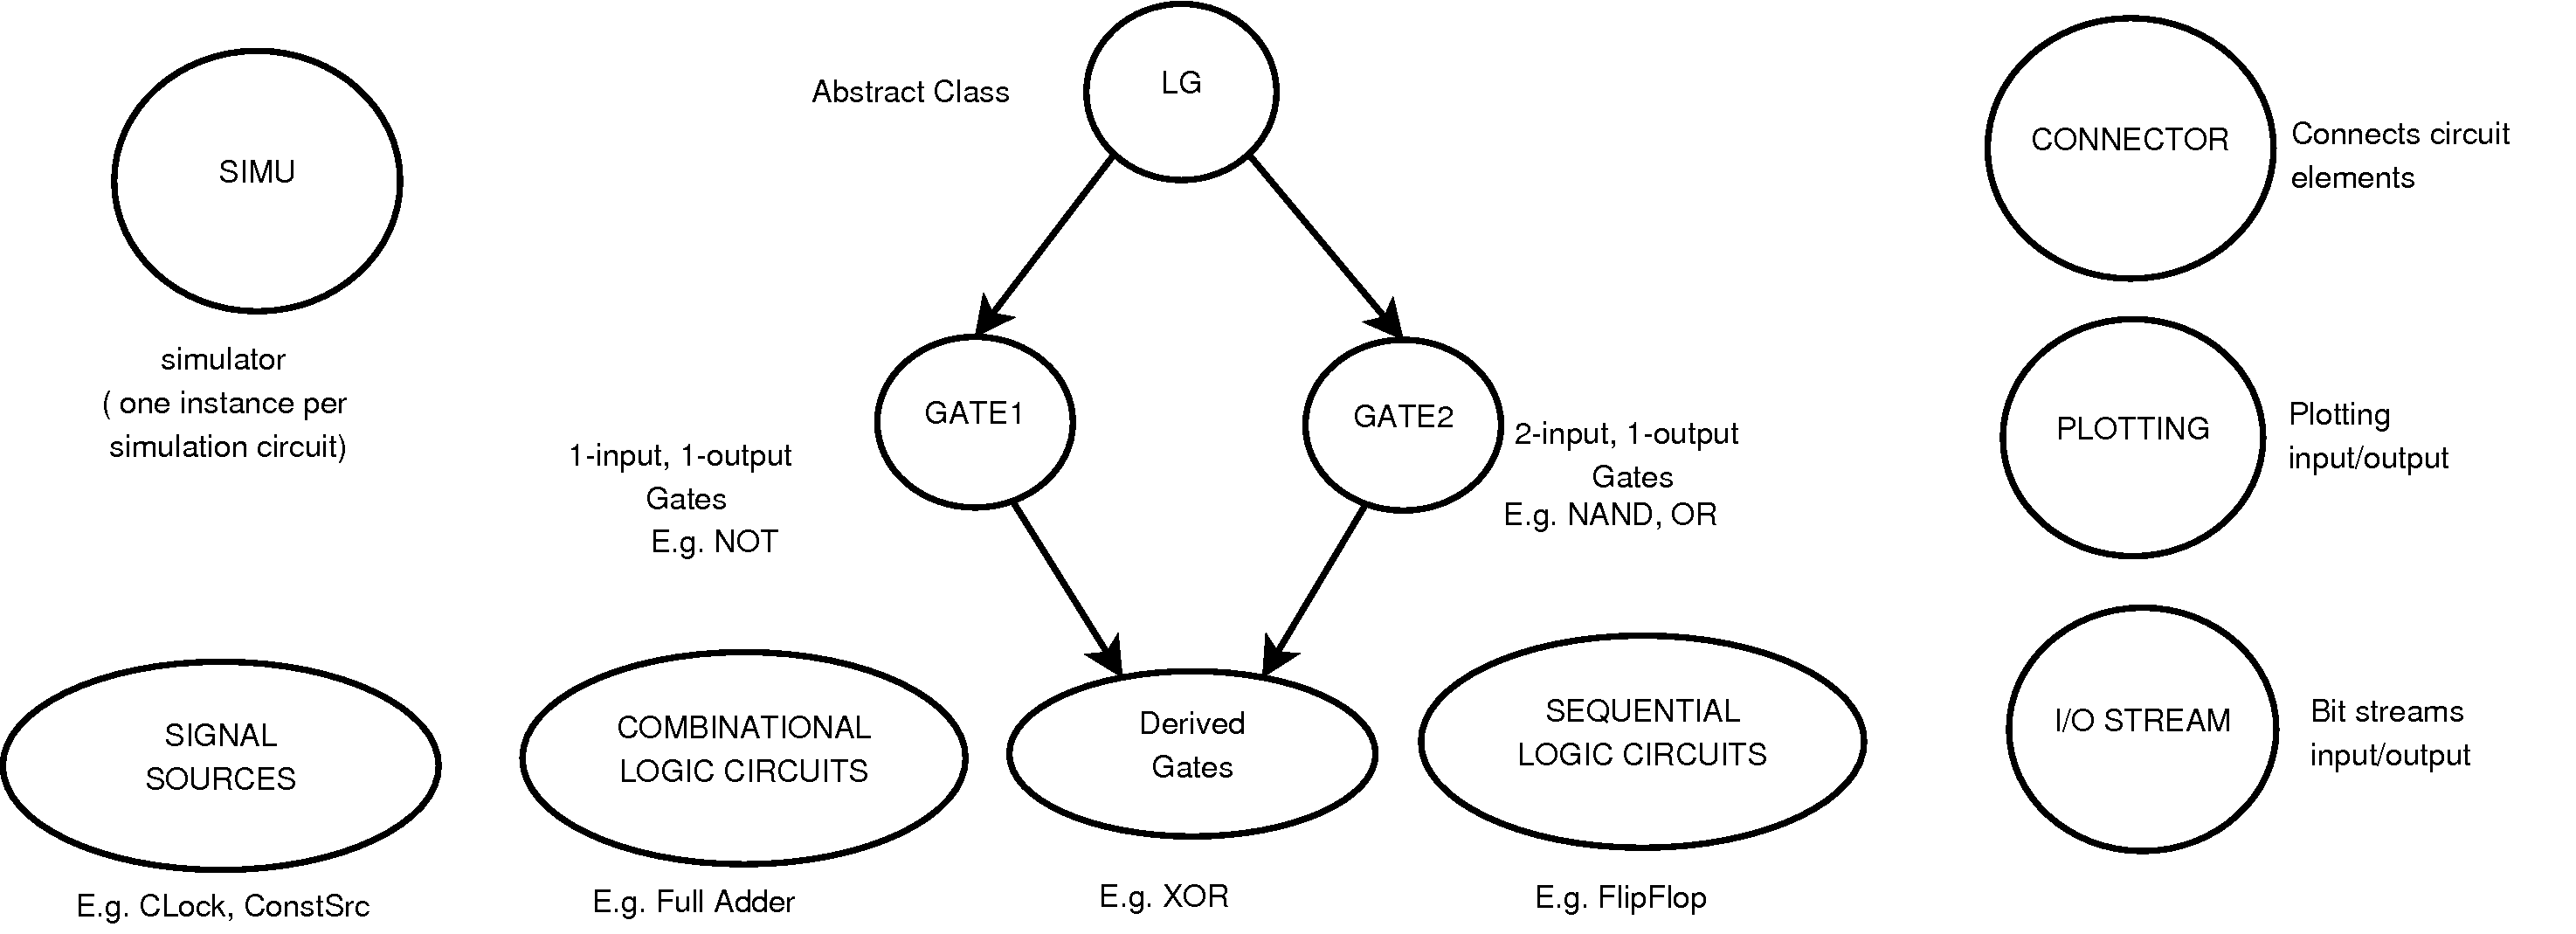
\includegraphics[scale=0.25]{class3.png}
   \caption{\scriptsize{Class Structure }}
  \end{center}
  \end{figure}

\end{frame}


\begin{frame}
 \frametitle{Implementation Details - Simulator Model}
  \begin{figure}
   \begin{center}
   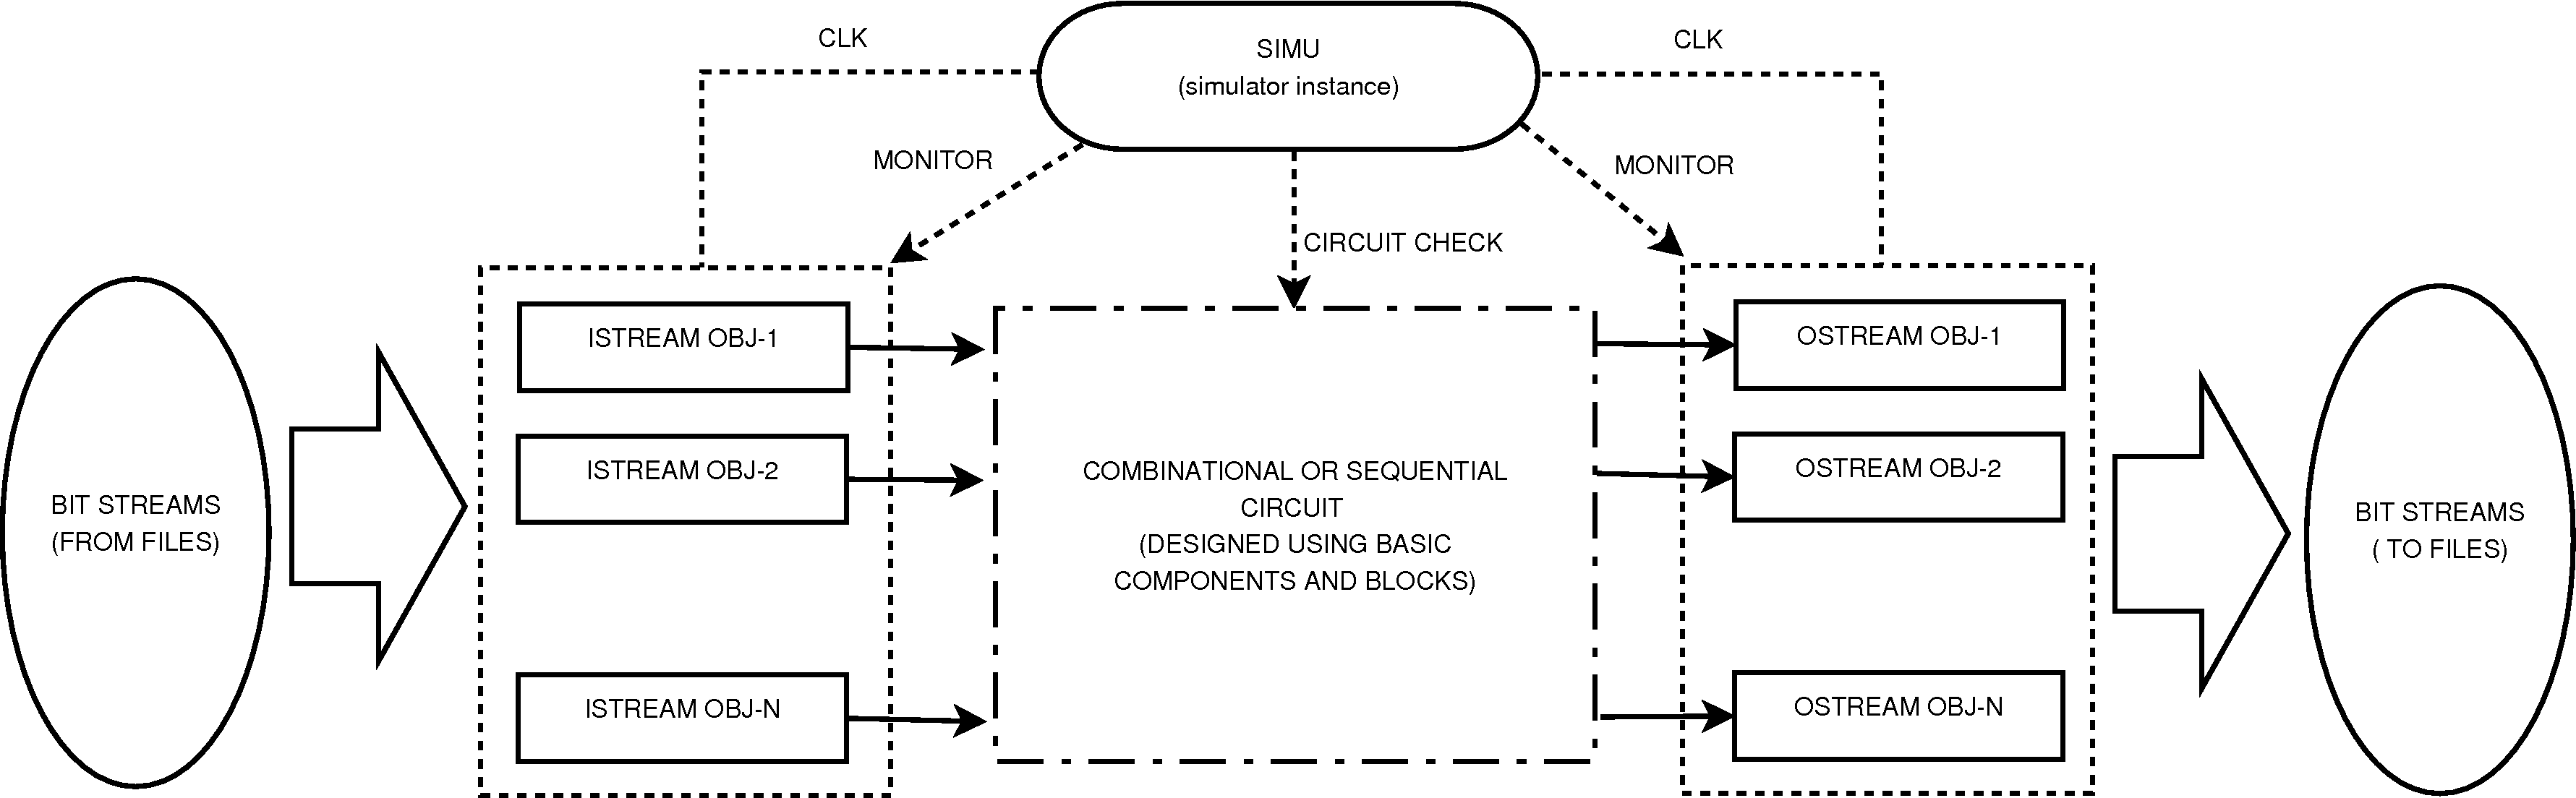
\includegraphics[scale=0.2]{syst_model.png}
   \caption{\scriptsize{Simulator model }}
  \end{center}
  \end{figure}

\end{frame}



\begin{frame}

 \frametitle{Implementation Details - Simulator Model}

  \begin{figure}
   \begin{center}
   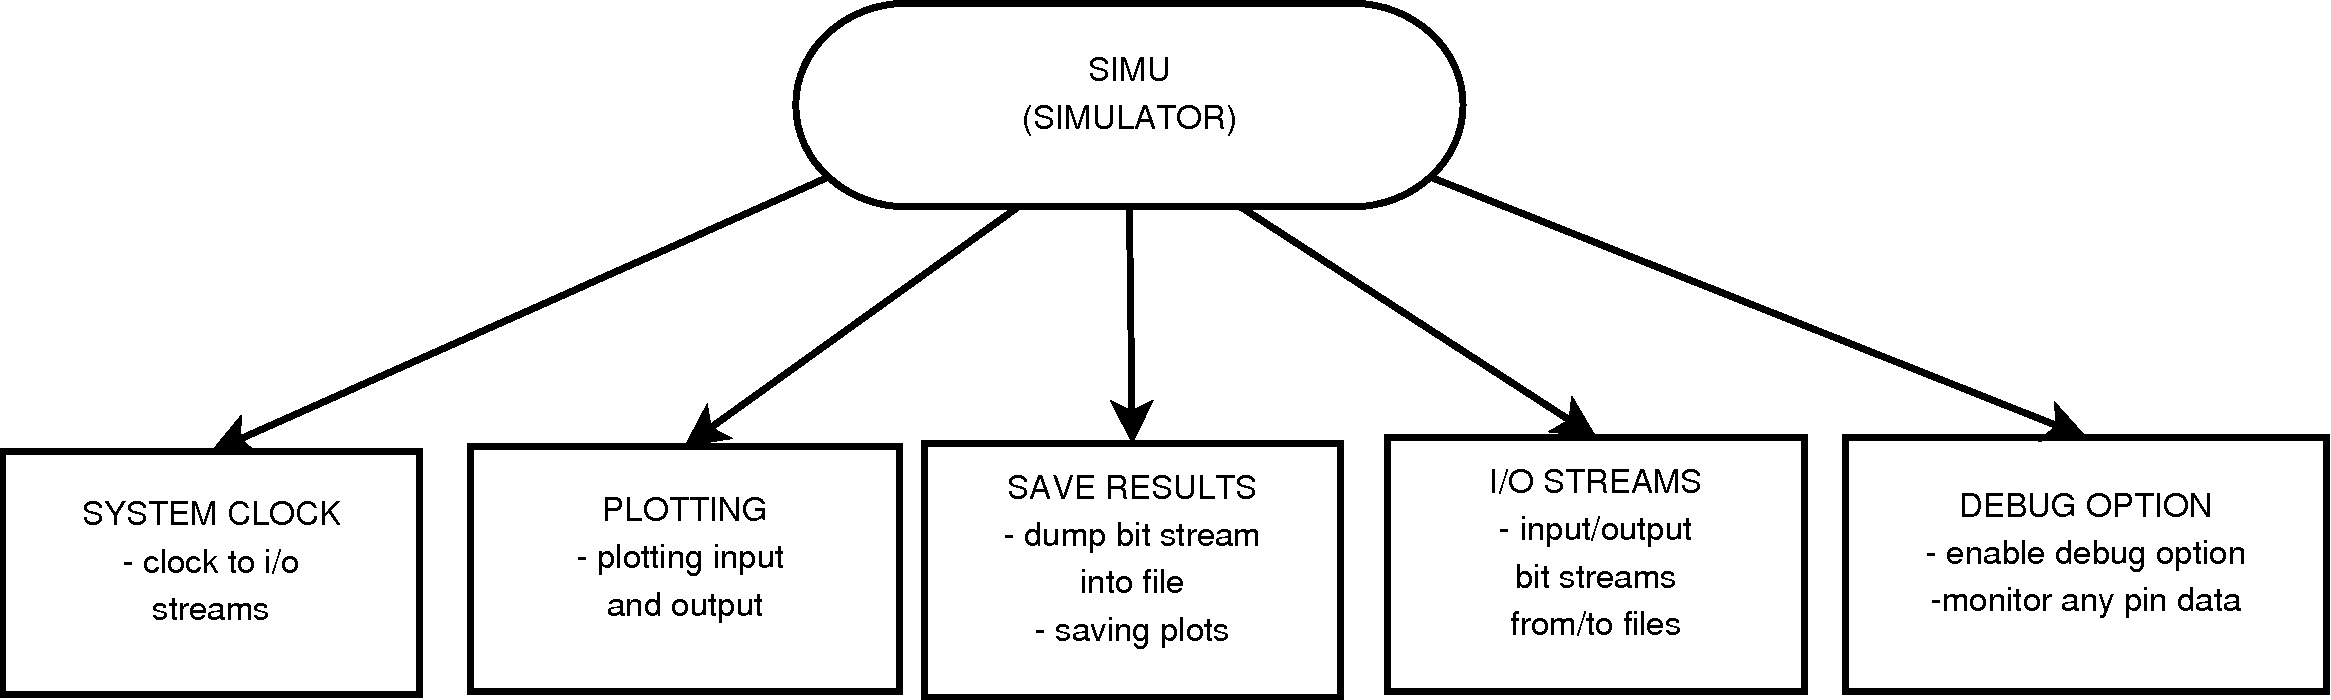
\includegraphics[scale=0.2]{simu_model.png}
    \caption{\scriptsize{\emph{SIMU} Class details }}
  \end{center}
  \end{figure}



 \begin{figure}
   \begin{center}
   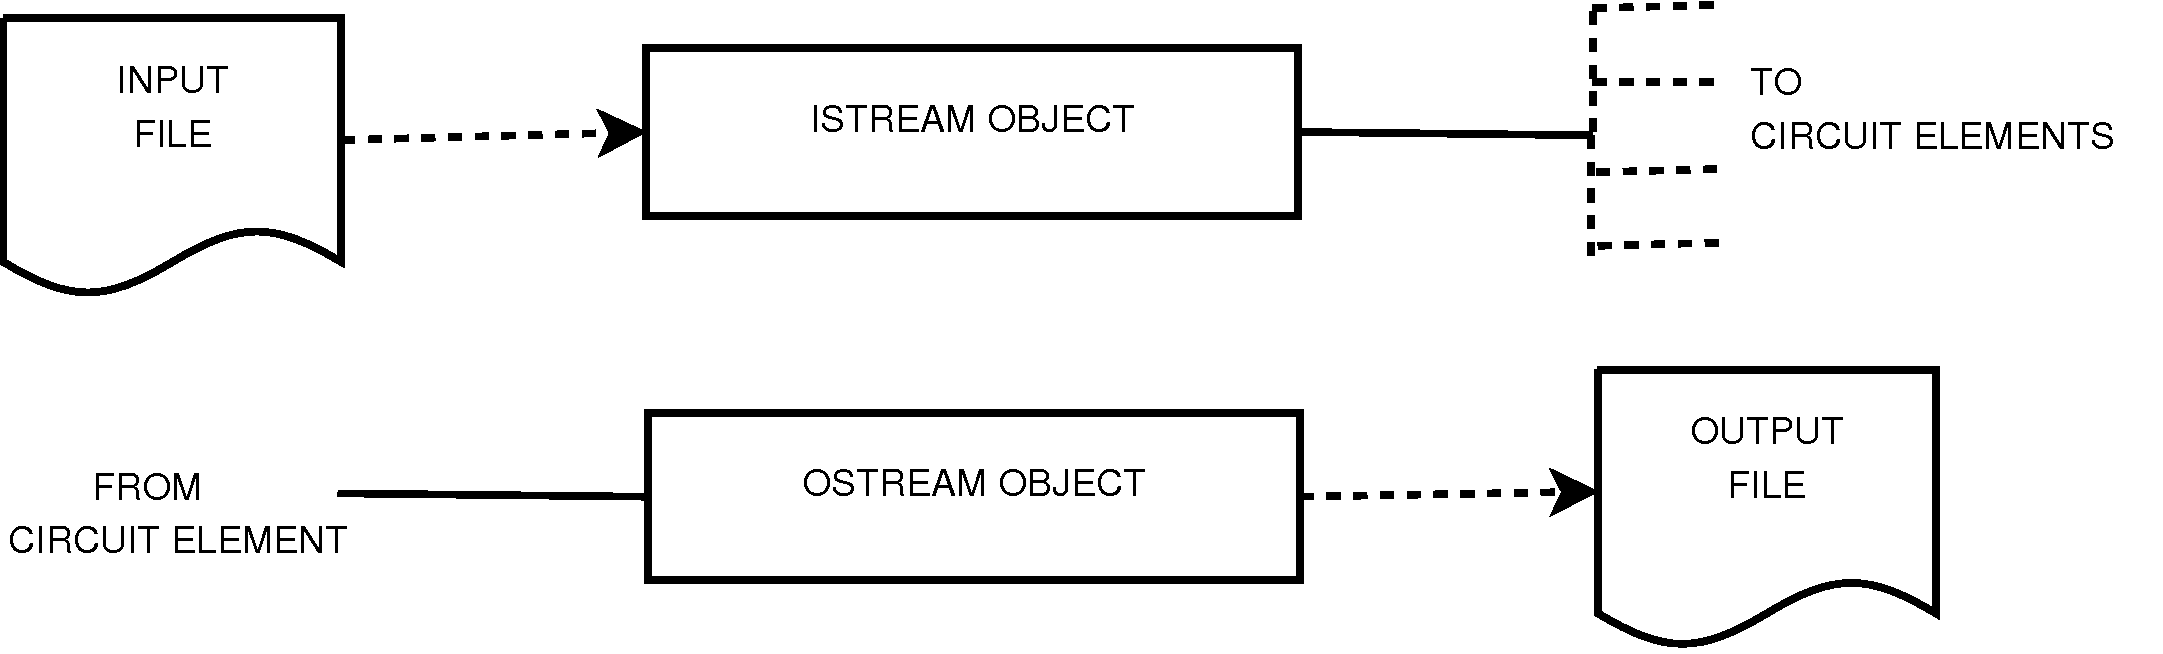
\includegraphics[scale=0.2]{iostream.png}
    \caption{\scriptsize{\emph{i/o stream} model }}
  \end{center}
  \end{figure}

\end{frame}





\begin{frame}
 \frametitle{Coding Details - Basic Gates}

\begin{block}<+->{Logic Gate Class - Abstract Class}

\begin{listing}
 %\centering
%  \caption{\scriptsize{Example output for GET/SET HDLC frame size}}
 \lstinputlisting[language=]{lg_code.py}
\end{listing}

\end{block}

\begin{block}<+->{AND Gate}
\begin{listing}
 %\centering
%  \caption{\scriptsize{Example output for GET/SET HDLC frame size}}
 \lstinputlisting[language=]{and_code.py}
\end{listing}

\end{block}

\end{frame}


\begin{frame}
 \frametitle{Coding Details - Derived  Gates}

\begin{block}<+->{XOR Gate}

\begin{listing}
 %\centering
%  \caption{\scriptsize{Example output for GET/SET HDLC frame size}}
 \lstinputlisting[language=]{xor_code.py}
\end{listing}

\end{block}


\end{frame}


\begin{frame}
 \frametitle{Coding Details - Sequential Element}

\begin{block}<+->{T Flip Flop}

\begin{listing}
 %\centering
%  \caption{\scriptsize{Example output for GET/SET HDLC frame size}}
 \lstinputlisting[language=]{t_code.py}
\end{listing}

\end{block}


\end{frame}


\begin{frame}
 \frametitle{Example Circuit Simulation - Circuit}
\begin{figure}
   \begin{center}
   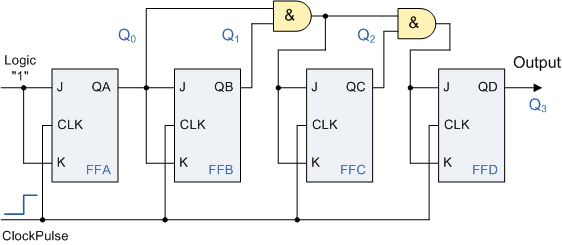
\includegraphics[scale=0.33]{cou4.png}
    \caption{\scriptsize{Example - 4 Bit synchronous binary counter }}
  \end{center}
  \end{figure}

\end{frame}

\begin{frame}
 \frametitle{Example Circuit Simulation - Code}

\begin{block}<+->{}

\begin{listing}
 %\centering
%  \caption{\scriptsize{Example output for GET/SET HDLC frame size}}
 \lstinputlisting[language=]{cou4.py}
\end{listing}

\end{block}


\end{frame}


\begin{frame}
 \frametitle{Example Circuit Simulation - Plots}
\begin{figure}
   \begin{center}
   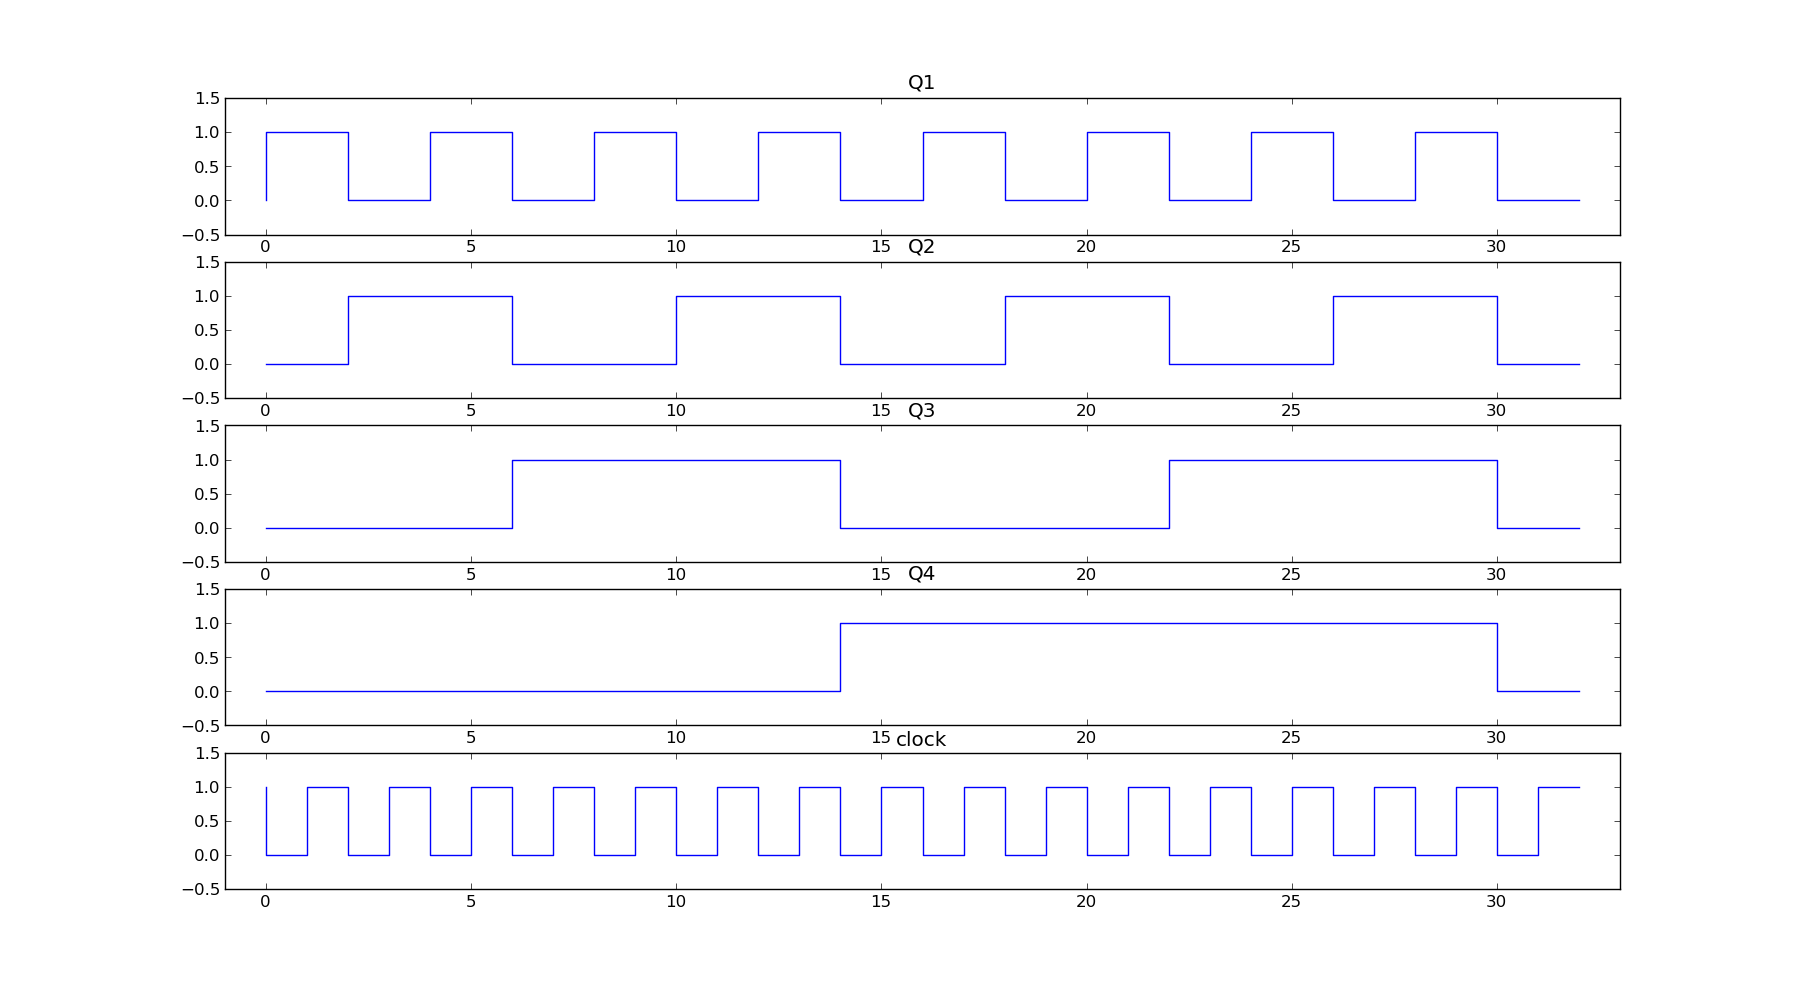
\includegraphics[scale=0.25]{cou44.png}
    \caption{\scriptsize{Example - 4 Bit synchronous binary counter plot}}
  \end{center}
  \end{figure}

\end{frame}


\begin{frame}
 \frametitle{Project Status \& future work}

\begin{block}<+->{Project Status}

\begin{itemize}
 \item Project status - Complete as per proposal
 \item Work hours put - approximately 25 hours per person 
\end{itemize}

\end{block}

\begin{block}<+->{Future Work}

\begin{itemize}
 \item GUI is not provided completely, so this could be potential future work.
 \item Feedback that activates the evaluation function is not possible in current release, this problem could be rectified.
\end{itemize}

\end{block}






\end{frame}



\begin{frame}

\centering{\Large{Thank You !}}


\end{frame}


%==========================================================================
% 
% \begin{frame}
%  \frametitle{Issues and Status}
% 
% \begin{block}<+->{Issues/Difficulties}
%  \begin{itemize}
% %   \item Connecting different Gates
%   \item Textual representation of circuit schematic
%   \item Tracking the signal propagation - event driven, multi-tier circuit
%   \item Managing connection between combinational and sequential circuit elements
%   \item Detection of floating pins
% %   \item 
%  \end{itemize}
% 
% \end{block}
% 
% 
% % Status
% 
% \begin{block}<+->{Project Status}
% \begin{itemize}
%  \item Approximately 20$\%$ work is done
%  \item Number of hours put : 3 hours per person
% \end{itemize}
% \end{block}
% 
% \end{frame}



\end{document}
